% Options for packages loaded elsewhere
\PassOptionsToPackage{unicode}{hyperref}
\PassOptionsToPackage{hyphens}{url}
%
\documentclass[10pt,a4paper]{article}
\usepackage[left=25mm,right=25mm]{geometry}

\usepackage{amsmath,amssymb}
\usepackage{lmodern}
\usepackage{iftex}
\ifPDFTeX
  \usepackage[T1]{fontenc}
  \usepackage[utf8]{inputenc}
  \usepackage{textcomp} % provide euro and other symbols
\else % if luatex or xetex
  \usepackage{unicode-math}
  \defaultfontfeatures{Scale=MatchLowercase}
  \defaultfontfeatures[\rmfamily]{Ligatures=TeX,Scale=1}
\fi
% Use upquote if available, for straight quotes in verbatim environments
\IfFileExists{upquote.sty}{\usepackage{upquote}}{}
\IfFileExists{microtype.sty}{% use microtype if available
  \usepackage[]{microtype}
  \UseMicrotypeSet[protrusion]{basicmath} % disable protrusion for tt fonts
}{}
\makeatletter
\@ifundefined{KOMAClassName}{% if non-KOMA class
  \IfFileExists{parskip.sty}{%
    \usepackage{parskip}
  }{% else
    \setlength{\parindent}{0pt}
    \setlength{\parskip}{6pt plus 2pt minus 1pt}}
}{% if KOMA class
  \KOMAoptions{parskip=half}}
\makeatother
\usepackage{xcolor}
\usepackage{longtable,booktabs,array}
\usepackage{multirow}
\usepackage{calc} % for calculating minipage widths
% Correct order of tables after \paragraph or \subparagraph
\usepackage{etoolbox}
\makeatletter
\patchcmd\longtable{\par}{\if@noskipsec\mbox{}\fi\par}{}{}
\makeatother
% Allow footnotes in longtable head/foot
\IfFileExists{footnotehyper.sty}{\usepackage{footnotehyper}}{\usepackage{footnote}}
\makesavenoteenv{longtable}
\usepackage{graphicx}
\makeatletter
\def\maxwidth{\ifdim\Gin@nat@width>\linewidth\linewidth\else\Gin@nat@width\fi}
\def\maxheight{\ifdim\Gin@nat@height>\textheight\textheight\else\Gin@nat@height\fi}
\makeatother
% Scale images if necessary, so that they will not overflow the page
% margins by default, and it is still possible to overwrite the defaults
% using explicit options in \includegraphics[width, height, ...]{}
\setkeys{Gin}{width=\maxwidth,height=\maxheight,keepaspectratio}
% Set default figure placement to htbp
\makeatletter
\def\fps@figure{htbp}
\makeatother
\setlength{\emergencystretch}{3em} % prevent overfull lines
\providecommand{\tightlist}{%
  \setlength{\itemsep}{0pt}\setlength{\parskip}{0pt}}
\setcounter{secnumdepth}{-\maxdimen} % remove section numbering
\ifLuaTeX
  \usepackage{selnolig}  % disable illegal ligatures
\fi
\IfFileExists{bookmark.sty}{\usepackage{bookmark}}{\usepackage{hyperref}}
\IfFileExists{xurl.sty}{\usepackage{xurl}}{} % add URL line breaks if available
\urlstyle{same} % disable monospaced font for URLs
\hypersetup{
  hidelinks,
  pdfcreator={LaTeX via pandoc}}

\author{}
\date{}

\begin{document}

\begin{quote}
EE 435\\
Homework 1\\
Spring 2024\\
Due Wednesday Jan 24

Problem 1 Identify one operational amplifier that has been published in
one of the following in the past 5 years:\\
IEEE Journal of Solid State Circuits\\
IEEE Trans. On Circuits and Systems (Part 1 or Part 2)\\
IEEE International Symposium on Circuits and Systems

Give the circuit schematic, citation information, and briefly summarize
the useful properties that the author claims for the circuit that you
identify.


The operational amplifier that I found was from the \textit{Design and Analysis of Two-Stage CMOS Operational Amplifier for Fluorescence Signal Processing}\ref{opamp} paper. This was published in the IEEE in the Journal of Solid State Circuits. In this paper it describes a operational amplifier for use in 


Problem 2 Identify one operational amplifier that has been patented in
the past 5 years. Give the circuit schematic, patent number, and briefly
summarize the useful properties that the author claims for this circuit.

The operational amplifier that I found was from Texas Instruments that is still pending from its application on 2023-02-16.



Schematic:
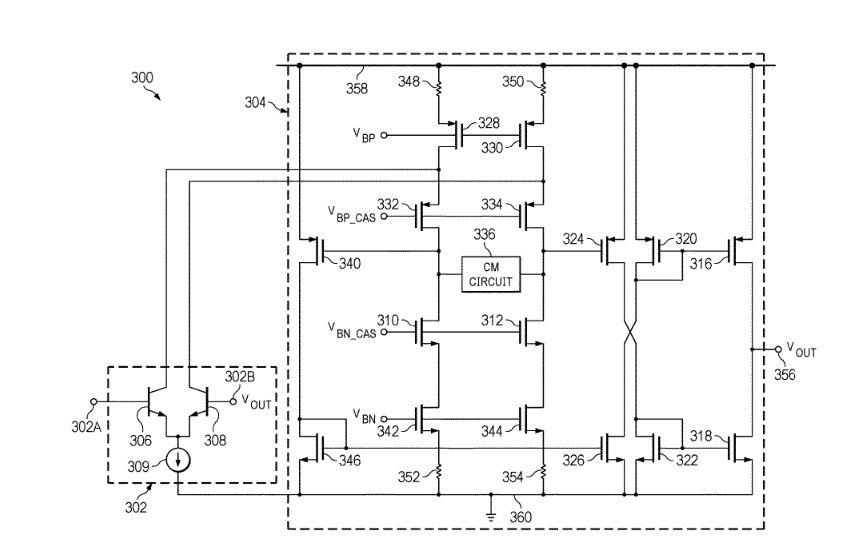
\includegraphics[width=3.61111in,height=2.58333in]{images/TIOpAmpSchematic.png}
Patent Number: US20230051462A1


Problem 3 A block diagram of what is often termed a voltage-series
feedback amplifier1 is shown below where it is assumed that the forward
A amplifier is a voltage amplifier with an input impedance of RIN, an
output impedance of R0 and a forward voltage gain of AV. The internal
feedback amplifier, denoted with the symbol β, is assumed to be an ideal
voltage amplifier (likely an attenuator) with infinite input impedance
and zero output impedance with feedback signal \textbf{V} F = β
\textbf{V} OUT . The

desensitivity, D, of a feedback amplifier is defined by the expression D
= + A V β . The

voltage gain AV can itself be frequency dependent and modeled by the
expression
\end{quote}



\begin{quote}
bandwidth of the forward amplifier.

Under these assumptions, show analytically that\\
a)The input impedance of the feedback amplifier is improved by D (i.e.

RINF=RIN•D)\\
b)The output impedance of the feedback amplifier is improved by D (i.e.

ROF=RO/D)\\
c)The closed loop bandwidth is improved by D (i.e. BWFB=BW*D)
\end{quote}




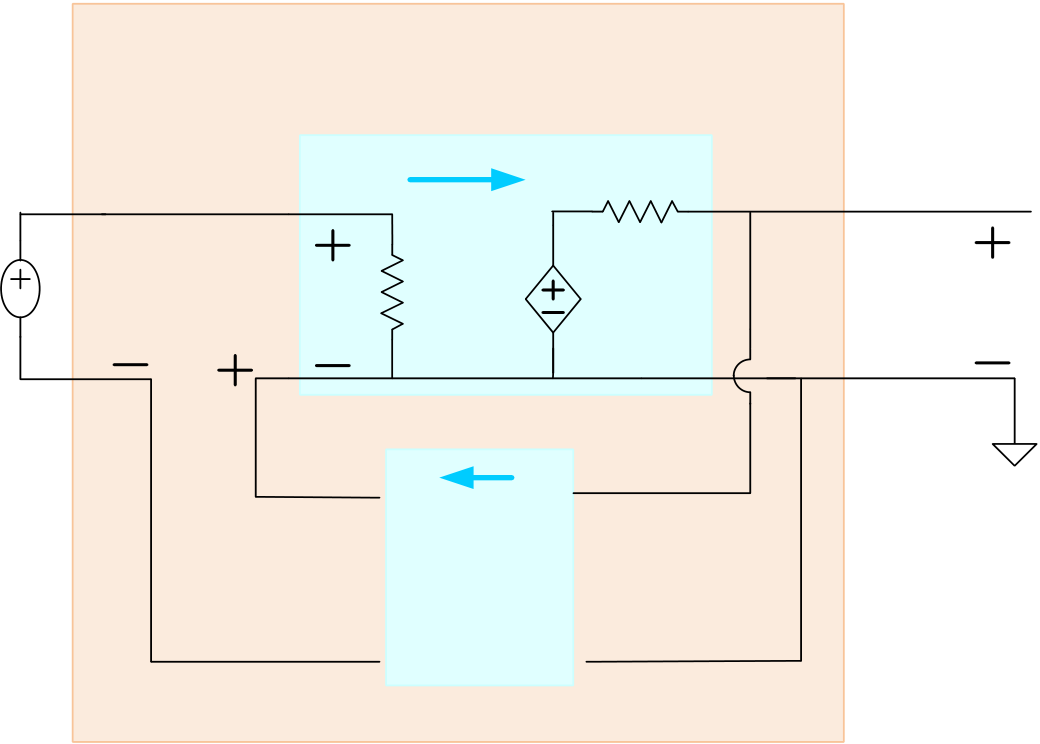
\includegraphics[width=3.61111in,height=2.58333in]{vertopal_3376d9a0695b4078a59040ba2f51c60d/media/image1.png}


\begin{quote}
Note: The improvements in this amplifier appear to be dramatic since the
desensitivity D can be very large. But the improvements might not be
quite as good as the calculations suggest since the assumptions of
ideality of the β amplifier may be difficult to completely meet and
because it may be difficult to get perfect summing of VIN and VF. But in
good feedback designs, the improvements in these parameters can be
really significant.

Notation associated with feedback amplifiers is often a bit cumbersome
since the whole structure comprised of the ``A'' and ``β'' networks is
often called a feedback amplifier. And internal to this structure, there
is a ``β'' network which is an amplifier that provides a feedback signal
so it is often referred to as a feedback amplifier as well. In this
problem, the term ``feedback amplifier'' will refer to the whole
structure and ``local feedback amplifier'' will refer to the ``β''
network to avoid possible confusion.

Problem 4 In the previous problem, feedback was used to build a voltage
feedback amplifier with improvements in four key characteristics.
Consider now the current feedback amplifier shown below where it is
assumed that the β amplifier is an ideal current amplifier with zero
input impedance and infinite output impedance characterized by the
equation F = β i OUT . The desensitivity is now defined by the
expression

D = + A I β . Express RINF in terms of the desensitivity and the
parameters in the

feedback amplifier and comment on these results relative to what was
obtained for the voltage feedback amplifier in the previous problem.
\end{quote}


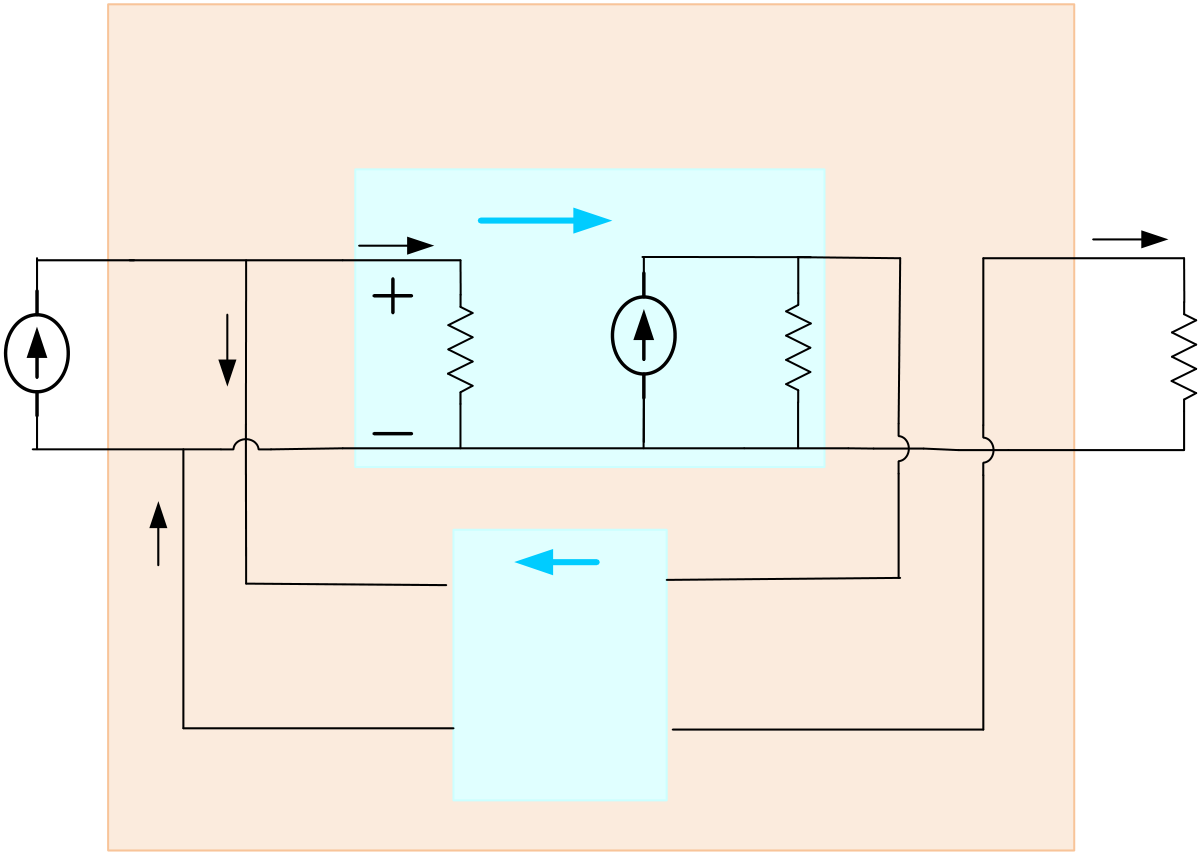
\includegraphics[width=4.16667in,height=2.95833in]{vertopal_3376d9a0695b4078a59040ba2f51c60d/media/image2.png}

\begin{quote}
Feedback Amplifier
\end{quote}



\begin{quote}
\textbf{i}F
\end{quote}

β

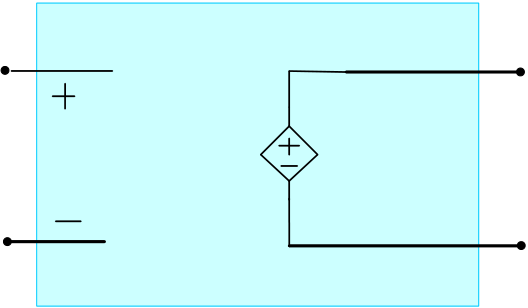
\includegraphics[width=1.83333in,height=1.06944in]{vertopal_3376d9a0695b4078a59040ba2f51c60d/media/image7.png}

\begin{quote}
Problem 5 In most texts, data sheets, and circuit schematics the
operational amplifier is represented as a 3-terminal device yet the
two-port model of an operational amplifier has 4 terminals (i.e. nodes)
as shown below. It thus appears that one terminal has somehow vanished
in the symbol or equivalently appeared in the two-port model.

Correspondingly, the model of the operational amplifier that is
described in the most recent version of the Sedra-Smith text shows four
terminals (one designated with the ground symbol) yet this ground
terminal does not appear to be on the op amp symbol or on the pinout of
the operational amplifiers we are using in the laboratory. Rigorously
reconcile this concept of the vanishing terminal!
\end{quote}



Ideal Voltage Amplifier

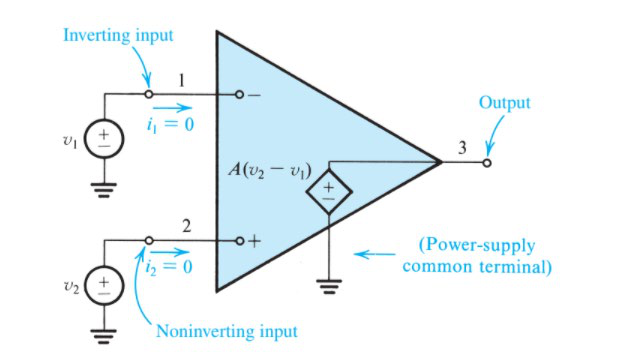
\includegraphics[width=2.99028in,height=1.71667in]{vertopal_3376d9a0695b4078a59040ba2f51c60d/media/image5.png}

\begin{quote}
Problem 6 The actual op amp is a five-terminal device. After reconciling
this issue of the vanishing terminal in the previous problem, give an
expression for the nodal output voltage with respect to VSS for the
operational amplifier shown below which explicitly shows the 5 terminals
of the device.
\end{quote}

\begin{longtable}[]{@{}
  >{\raggedright\arraybackslash}p{(\columnwidth - 4\tabcolsep) * \real{0.3333}}
  >{\raggedright\arraybackslash}p{(\columnwidth - 4\tabcolsep) * \real{0.3333}}
  >{\raggedright\arraybackslash}p{(\columnwidth - 4\tabcolsep) * \real{0.3333}}@{}}
\toprule()
\multirow{2}{*}{\begin{minipage}[b]{\linewidth}\raggedright
Problem 7
\end{minipage}} & \begin{minipage}[b]{\linewidth}\raggedright
\begin{quote}
V2\\
V1
\end{quote}\strut
\end{minipage} & \begin{minipage}[b]{\linewidth}\raggedright
\begin{quote}
VDD

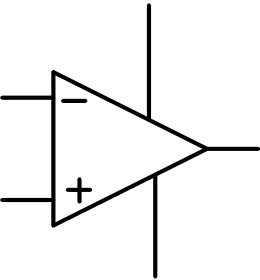
\includegraphics[width=0.90278in,height=0.97222in]{vertopal_3376d9a0695b4078a59040ba2f51c60d/media/image6.png}VOUT

VSS
\end{quote}
\end{minipage} \\
&
\multicolumn{2}{>{\raggedright\arraybackslash}p{(\columnwidth - 4\tabcolsep) * \real{0.6667} + 2\tabcolsep}@{}}{%
\begin{minipage}[b]{\linewidth}\raggedright
\begin{quote}
Two circuits that use a single operational amplifier are shown below.
\end{quote}
\end{minipage}} \\
\midrule()
\endhead
\bottomrule()
\end{longtable}

\begin{quote}
a)Using the model of the standard model of the operational amplifier
that appears in the Sedra/Smith book, analyze the two circuits under the
assumption that the voltage gain of the op amp, AV, is finite.
\end{quote}

b)Compare the voltage gain of the two circuits as the voltage gain AV
goes to ∞

Page 4

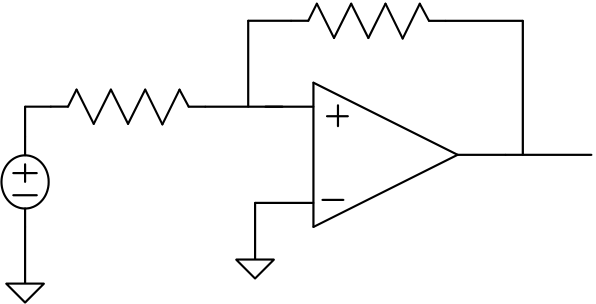
\includegraphics[width=2.06944in,height=1.05556in]{vertopal_3376d9a0695b4078a59040ba2f51c60d/media/image8.png}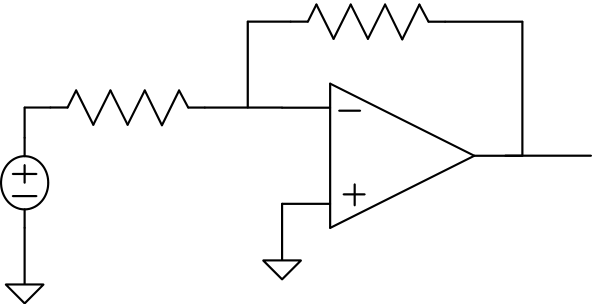
\includegraphics[width=2.05556in,height=1.05556in]{vertopal_3376d9a0695b4078a59040ba2f51c60d/media/image9.png}

\begin{quote}
c)Although an engineer should be able to analyze any interconnection of
basic devices and components, almost all basic electronics textbooks are
silent on the existence of the simple circuit on the right. Why is this
circuit is seldom discussed? Support your answer with sound analytical
principles or concepts.
\end{quote}

\begin{longtable}[]{@{}
  >{\raggedright\arraybackslash}p{(\columnwidth - 4\tabcolsep) * \real{0.3333}}
  >{\raggedright\arraybackslash}p{(\columnwidth - 4\tabcolsep) * \real{0.3333}}
  >{\raggedright\arraybackslash}p{(\columnwidth - 4\tabcolsep) * \real{0.3333}}@{}}
\toprule()
\multirow{3}{*}{\begin{minipage}[b]{\linewidth}\raggedright
\begin{quote}
R2 R1

VIN
\end{quote}

Problem 8 (Extra Credit)
\end{minipage}} &
\multicolumn{2}{>{\raggedright\arraybackslash}p{(\columnwidth - 4\tabcolsep) * \real{0.6667} + 2\tabcolsep}@{}}{%
\begin{minipage}[b]{\linewidth}\raggedright
\begin{quote}
R2\\
R1
\end{quote}\strut
\end{minipage}} \\
& \begin{minipage}[b]{\linewidth}\raggedright
\begin{quote}
VOUT
\end{quote}
\end{minipage} & \begin{minipage}[b]{\linewidth}\raggedright
VOUT
\end{minipage} \\
&
\multicolumn{2}{>{\raggedright\arraybackslash}p{(\columnwidth - 4\tabcolsep) * \real{0.6667} + 2\tabcolsep}@{}}{%
\begin{minipage}[b]{\linewidth}\raggedright
VIN

\begin{quote}
One example was given in class where Conventional
\end{quote}
\end{minipage}} \\
\midrule()
\endhead
\bottomrule()
\end{longtable}

\begin{quote}
Wisdom does not correctly reflect reality and that was in describing the
concept of the operational amplifier. Another example, also related to
operational amplifiers, is the ``vanishing ground'' of Problem 5 in this
homework assignment. See if you can identify another example, preferably
in the electronics field, where Conventional Wisdom is not correctly
aligned with reality.
\end{quote}

\begin{thebibliography}{9}
\bibitem{opamp}\href{https://ieeexplore.ieee.org/document/9532225}{Design and Analysis of Two-Stage CMOS Operational Amplifier for Fluorescence Signal Processing}

\end{thebibliography}

\end{document}
